

% Morten -- jeg skriver bare en veldig plain tex-fil her, så kan du gjøre det du vil med innholdet etterpå.


\documentclass{article}
\usepackage[utf8]{inputenc}
\usepackage[a4paper]{geometry}
\usepackage[norsk]{babel}
\usepackage{amssymb}
\usepackage{amsmath}
\usepackage{amsthm}
\usepackage{multicol}
\usepackage{scrextend}
\usepackage{mdframed}
\usepackage{hyperref}
\usepackage{listings}
\usepackage{tikz}
\usetikzlibrary{patterns,decorations.pathmorphing, decorations.pathreplacing}
\usepackage{pgfplots}
\usepackage{array}
\usepackage{mdframed}
\usepackage[american]{circuitikz}
\usepackage[small]{titlesec}

\hypersetup{colorlinks=true, 
    linkcolor=blue, 
    filecolor=magneta,
    urlcolor=cyan,
    citecolor=black,
}

\setlength{\parindent}{0em}
\setlength{\parskip}{1em}

\theoremstyle{plain}
\newtheorem{thm}{Teorem}\surroundwithmdframed{thm}
\newtheorem{prop}[thm]{Proposisjon}

\theoremstyle{definition}
\newtheorem{defnx}[thm]{Definisjon}
\newtheorem{exx}[thm]{Eksempel}
\newtheorem{bevisskisse}[thm]{Skisse av bevis}

\theoremstyle{remark}
\newtheorem{remarkx}[thm]{Merknad}

\newenvironment{defn}
{\pushQED{\qed}\renewcommand{\qedsymbol}{$\triangle$}\defnx}
{\popQED\enddefnx}
\newenvironment{ex}
{\pushQED{\qed}\renewcommand{\qedsymbol}{$\triangle$}\exx}
{\popQED\endexx}
\newenvironment{remark}
{\pushQED{\qed}\renewcommand{\qedsymbol}{$\triangle$}\remarkx}
{\popQED\endremarkx}


% Endre på disse etter hvilken notasjon du vil ha.
\newcommand{\diff}[1]{\mathop{d#1}}
\newcommand{\fcn}{x}
\newcommand{\boldvec}[1]{\boldsymbol{\mathrm{#1}}}
\newcommand{\expfcn}[1]{e^{#1}}
\newcommand{\abs}[1]{|#1|}
\newcommand{\bigabs}[1]{\big|#1\big|}
\newcommand{\biggabs}[1]{\bigg|#1\bigg|}
\newcommand{\bigparanth}[1]{\big(#1\big)}
\newcommand{\biggparanth}[1]{\bigg(#1\bigg)}
\newcommand{\bigbrac}[1]{\big[#1\big]}
\newcommand{\biggbrac}[1]{\bigg[#1\bigg]}
\newcommand{\imagunit}{\mathrm{j}}
\newcommand{\bigo}[1]{O(#1)}

\DeclareMathOperator{\imaginary}{Im}
\DeclareMathOperator{\real}{Re}


\title{Førsteordens ordinære differensialligninger}
\author{}
\date{}

\begin{document}
\maketitle

Dette kapittelet gir en introduksjon til førsteordens ordinære differensialligninger. For lineære differensialligninger finnes det god teori og universelle løsningsteknikker, og vi kan ofte finne analytiske løsninger for disse. Dette gjelder i mye mindre grad for ikke-lineære differensialligninger, som det ofte er mye vanskeligere å utlede analytiske løsninger til, og som vi er avhengig av kvalitative eller numeriske metoder for å kunne analysere.

Vi begynner med å se på noen eksempler hvor differensialligninger oppstår som modeller for fysiske situasjoner, og kommer deretter tilbake til hvordan vi kan finne løsninger og forstå dynamikken bak modellene.

\begin{ex} \label{eks:krets_1}
    Følgende figur viser en elektrisk krets med en spenningskilde, en motstand og en spole (RL-krets).
    \begin{center}
        \begin{circuitikz}
            \draw
            (0,0)
            to[american voltage source, voltage dir=old, l={$V_s(t)$}, i^={$I(t)$}] (0,3)
            to[european resistor, l_ = $R$] (3,3)
            to (3,0)
            to[cute inductor, l_ = $L$] (0, 0);
        \end{circuitikz}
    \end{center}
    Ved Ohms lov er spenningsfallet over motstanden lik $RI$ og spenningsfallet over spolen er $L\dot{I}$, der $I(t)$ er strømmen i kretsen som funksjon av tid. Kirchhoffs spenningslov, som sier at summen av potensialforskjellene over en lukket strømsløyfe må utligne hverandre, gir dermed at
    \begin{equation*}
        \dot{I} + \frac{R}{L} I = \frac{V_s}{L}.
    \end{equation*}
    Dette er et eksempel på en førsteordens lineær og ordinær differensialligning, hvor vi er på jakt etter den ukjente funksjonen $I$.
\end{ex}

\begin{ex} \label{eks:populasjon_1}
    I studiet av populasjonsvekst møter man ofte den logistiske ligningen
    \begin{equation*}
        \dot{\fcn}(t) = A \fcn(t) - B (\fcn(t))^2,
    \end{equation*}
    hvor $\fcn(t)$ beskriver en populasjonsstørrelse som funksjon av tid. Dersom vi setter $B = 0$ får vi en malthusiansk modell, etter den britiske samfunnsøkonomen Thomas Robert Malthus. Rundt slutten av 1700-tallet hevdet Malthus at befolkningen i Europa ville øke eksponentielt samtidig som matproduksjonen ville øke lineært, noe som ville føre til befolkningskollaps gjennom sultkatastrofer og epidemier. Senere skal vi se at leddet $-B \fcn^2$ begrenser veksten i populasjonsmodellen, og bøter på Malthus' dystre fremtidsutsikter.
\end{ex}


\section*{En kort oversikt}

En førsteordens differensialligning er en relasjon mellom en (ukjent) funksjon og dens første deriverte. Vi skal i dette notatet bare jobbe med ordinære differensialligninger (forkortet som ODE (ordinary differential equation)); ligninger for funksjoner av én variabel. Generelt skal vi skrive førsteordens ODEer på formen
\begin{equation} \label{eq:generell_ekspl_forsteordens}
    \dot{\fcn}(t) = f(t, \fcn(t)),
\end{equation}
hvor $\dot{\fcn}$ betegner deriverte av funksjonen $\fcn$ med hensyn på variabelen $t$. Funksjonen $f$ beskriver relasjonen mellom $\dot{\fcn}(t)$, $t$ og $\fcn(t)$. Dersom $f$ ikke eksplisitt er avhengig av $t$, altså dersom vi kan skrive $f = f(\fcn(t))$, sier vi at ligningen er autonom. Videre, dersom $f$ er en lineær funksjon i $\fcn$ er ligningen lineær.

\begin{defn}
    Funksjonen $\fcn(t)$ er en løsning til ODEen \eqref{eq:generell_ekspl_forsteordens} på et åpent intervall $I = (a, b)$ dersom den er kontinuerlig deriverbar og tilfredsstiller ligningen på $I$.
\end{defn}

Vi har altså to krav for at et funksjon $x(t)$ skal være en løsning til \eqref{eq:generell_ekspl_forsteordens}. Først må funksjonen være deriverbar, og den deriverte må være kontinuerlig. Hvis ikke dette kravet er på plass gir ikke ligningen så mye mening. Videre må funksjonen naturligvis tilfredsstille ligningen. Det åpne intervallet $I$ kan være litt forvirrende, men nytten ligger i at vi nå kan snakke om løsninger som ikke nødvendigvis er definert på hele $\mathbb{R}$ (merk likevel at intervallet $I$ fint kan være hele $\mathbb{R}$).

\begin{ex}
    Ligningen
    \begin{equation*}
        \dot{x} = x^2
    \end{equation*}
    har løsning
    \begin{equation*}
        x(t) = \frac{1}{1-t}
    \end{equation*}
    på intervallet $(1, \infty)$. Siden $x(t)$ ikke eksisterer for $t=1$ kan løsningen ikke utvides til å gjelde på hele $\mathbb{R}$.
\end{ex}

Dersom det er mulig å finne et eksakt uttrykk ved hjelp av et endelig antall kjente funksjoner (polynomer, trigonometriske funksjoner, eksponentialfunksjoner, osv.) for løsningen til en differensialligning, sier man ofte at man har en analytisk løsning. Dette står i kontrast til numeriske løsninger, som er tilnærminger.

I modellering kommer differensialligninger sjelden uten betingelser som vi må ta hensyn til dersom vi skal løse dem. Initialverdiproblemer er eksempler på dette. Generelt kan vi skrive initialverdiproblemet for førsteordens ODEer som
\begin{equation} \label{eq:ivp}
    \left\{
    \begin{aligned}
            & \dot{\fcn} = f(t, \fcn), \\
            & \fcn(t_0) = \fcn_0,
    \end{aligned}
    \right.
\end{equation}
hvor $\fcn(t_0) = \fcn_0$ er initialbetingelsen. En vanlig fysisk tolkning av dette er at vi ønsker å finne banen til en partikkel som befinner seg i posisjonen $x_0$ ved tiden $t_0$, og hvis fart er bestemt av $\dot{\fcn} = f(t, \fcn)$.

La oss vri og vende litt på initialverdiproblemet gitt i \eqref{eq:ivp}. Husk hvordan derivasjon er definert; som grenseverdien av stigningen til en funksjon. På denne måten er ligning \eqref{eq:generell_ekspl_forsteordens} grensen til ligningen
\begin{equation*}
    \frac{\fcn(t + h) - \fcn(t)}{h} = f(t, \fcn(t)),
\end{equation*}
når $h \rightarrow 0$. På den annen side kan vi integrere \eqref{eq:ivp} fra $t_0$ til $t$, altså
\begin{equation*}
    \int_{t_0}^t \frac{\diff{}}{\diff{s}} \fcn(s) \diff{s} = \int_{t_0}^t f(s, \fcn(s)) \diff{s},
\end{equation*}
og bruke analysens fundamentalteorem på venstre side til å skrive ligningen på integralformen
\begin{equation} \label{eq:integralform}
    \fcn(t) = \fcn_0 + \int_{t_0}^{t} f(s, \fcn(s)) \diff{s}.
\end{equation}
Integrasjonen over er utført over en variabel $s$. Dette er naturligvis ikke substansielt for utregningen, siden $s$ forsvinner i integrasjonen, men det tillater oss å beholde variabelen $t$ i ligningen.

Integralet på høyre side av \eqref{eq:integralform} kan tilnærmes numerisk, noe som gir opphav til numeriske løsningsteknikker for initialverdiproblemet \eqref{eq:ivp}. En annen idé er å prøve fikspunktiterasjon på ligningen \eqref{eq:integralform}. Forhåpentligvis gir dette en smakebit på at differensialligninger kan (og bør) ses på i forskjellige lys, og at selv om det kan være vanskelig å utlede analytiske løsninger er det et stort utvalg av teknikker og triks tilgjengelig.


\section*{Lineære ligninger}

En førsteordens lineær ODE kan skrives på standard form som
\begin{equation} \label{eq:linear_forsteordens}
    \dot{\fcn}(t) + p(t) \fcn(t) = q(t),
\end{equation}
Dersom $q(t) = 0$ sier vi at ligningen er homogen. Ligning \eqref{eq:linear_forsteordens} kan faktisk løses generelt, som vist i følgende proposisjon.

\begin{prop} \label{prop:lineær_løsn}
    Anta at $p(t)$ og $q(t)$ er kontinuerlige funksjoner på et åpent intervall $I$ som inneholder punktet $t_0$. La $C$ være en konstant, og la $P(t)$ være en antiderivert av $p(t)$, altså
    \begin{equation*}
        P(t) = \int p(t) \diff{t}.
    \end{equation*}
    Da er funksjonen
    \begin{equation} \label{eq:generell_losn_linear}
        \fcn(t) = \expfcn{-P(t)} \biggparanth{ C + \int_{t_0}^t q(s) \expfcn{P(s)} \diff{s}},
    \end{equation}
    en generell løsning til ligning \eqref{eq:linear_forsteordens}.
\end{prop}

\begin{proof}[Bevis]
    Multiplikasjon med funksjonen $\expfcn{P(t)}$ på begge sider av ligning \eqref{eq:linear_forsteordens} gir
    \begin{equation*}
        \dot{\fcn}(t) \expfcn{P(t)} + \fcn(t) p(t) \expfcn{P(t)} = q(t) \expfcn{P(t)},
    \end{equation*}
    hvor vi har valgt $P(t)$ lik den antideriverte til $p(t)$. Ved kjerneregelen for derivasjon er venstre side nå lik den deriverte av $\fcn(t) \expfcn{P(t)}$, altså har vi
    \begin{equation*}
        \frac{\diff{}}{\diff{t}} \bigparanth{\fcn(t) \expfcn{P(t)}} = q(t) \expfcn{P(t)}.
    \end{equation*}
    Integrerer vi ligningen med hensyn på $t$ får vi
    \begin{equation*}
        \int_{t_0}^t \frac{\diff{}}{\diff{s}} \bigparanth{\fcn(s) \expfcn{P(s)}} \diff{s} = \int_{t_0}^{t} q(s) \expfcn{P(s)} \diff{s}.
    \end{equation*}
    Analysens fundamentalteorem gir da at
    \begin{equation*}
        \fcn(t) \expfcn{P(t)} - \fcn(t_0) \expfcn{P(t_0)} = \int_{t_0}^t q(s) \expfcn{P(s)} \diff{s},
    \end{equation*}
    hvor vi skriver $\fcn(t_0) \expfcn{P(t_0)}$ som en konstant $C$. Multiplikasjon med $\expfcn{-P(t)}$ på begge sider gir nå den generelle løsningen \eqref{eq:generell_losn_linear}.
\end{proof}

Løsningen kalles generell når den inneholder en ubestemt konstant $C$. Dersom konstanten $C$ bestemmes av initialbetingelser sier vi at vi har en spesiell løsning. La oss se på noen eksempler.

\begin{ex}
    Vi vet at ligningen
    \begin{equation*}
        \dot{\fcn} + a \fcn = 0
    \end{equation*}
    har generell løsning
    \begin{equation*}
        \fcn(t) = C \expfcn{-a t}
    \end{equation*}
    på hele $\mathbb{R}$. Dette stemmer overens med formelen \eqref{eq:generell_losn_linear} dersom vi setter $P(t) = \int a \diff{t} = at$ og $q(t) = 0$.
\end{ex}

\begin{ex} \label{eks:grundig_lineær}
    Vi løser ligningen
    \begin{equation*}
        \dot{\fcn} - 2\fcn = 3\expfcn{t}
    \end{equation*}
    med metoden fra Proposisjon \ref{prop:lineær_løsn} på hele $\mathbb{R}$. Her er $P(t) = \int -2 \diff{t} = -2t$, så vi ganger ligningen med $\expfcn{-2t}$, og får
    \begin{equation*}
        \dot{\fcn} \expfcn{-2t} - 2\fcn \expfcn{-2t} = 3\expfcn{t} \expfcn{-2t} = 3 \expfcn{-t}.
    \end{equation*}
    Dette kan vi forenkle til
    \begin{equation*}
        \frac{\diff{}}{\diff{t}} \bigparanth{\fcn \expfcn{-2t}} = 3 \expfcn{-t}
    \end{equation*}
    ved hjelp av kjerneregelen. Siden det ikke er oppgitt en initialbetingelse her kommer løsningen til å inneholde en ukjent konstant. Vi kan for eksempel integrere fra $0$ til $t$, som gir
    \begin{equation*}
        \begin{aligned}
            \int_0^t \frac{\diff{}}{\diff{s}} \bigparanth{\fcn(s) \expfcn{-2s}} \diff{s} & = \fcn(t)\expfcn{-2t} - \fcn(0) \\
            & = \int_0^t 3\expfcn{-s} \diff{s} = -3\expfcn{-t} + 3.
        \end{aligned}
    \end{equation*}
    Vi flytter så $x(0)$ over til høyre side og ganger med $\expfcn{2t}$, og står da igjen med den generelle løsningen
    \begin{equation*}
        \fcn(t) = (3+\fcn(0)) \expfcn{2t} - 3\expfcn{t} = C \expfcn{2t} - 3\expfcn{t}.
    \end{equation*}
    Den spesielle løsningen kan finnes ved å bestemme $C$ fra en initialbetingelse for problemet. Vi merker oss at funksjonen $\expfcn{2t}$ løser den homogene ligningen
    \begin{equation*}
        \dot{\fcn} - 2\fcn = 0,
    \end{equation*}
    og at funksjonen $-3\expfcn{t}$ løser den tilhørende inhomogene ligningen med $3\expfcn{t}$ på høyre side. Disse kalles henholdsvis den homogene og den inhomogene løsningen.
\end{ex}

\begin{ex} \label{eks:krets_2}
    La oss løse ligningen
    \begin{equation*}
        \dot{I} + \frac{R}{L} I = \frac{V_s}{L}
    \end{equation*}
    fra Eksempel \ref{eks:krets_1}, gitt at $V_s(t)$ er en kontinuerlig funksjon på et åpent intervall $I$. Proposisjon \ref{prop:lineær_løsn} gir da at den generelle løsningen for strømmen i kretsen er
    \begin{equation*}
        I(t) = \expfcn{-\frac{R}{L}t}\biggparanth{C + \int_{t_0}^t \frac{V_s(s)}{L} \expfcn{\frac{R}{L}s} \diff{s} }, 
    \end{equation*}
    for $t_0, t \in I$. Løsningen er naturligvis avhengig av spenningskilden $V_s(t)$.
\end{ex}

Med Proposisjon \ref{prop:lineær_løsn} kan vi løse en ganske stor klasse av førsteordens lineære ODEer. Her kommer et lite frempek på hvorfor vi har valgt å studere lineære ligninger som et eget tema før vi ser på ikke-lineære ligninger: de lineære teknikkene kan i stor grad generaliseres ved hjelp av lineær algebra.

Dersom funksjonen som inngår i ligningen er en vektorfunksjon med $n$ komponenter på formen
\begin{equation*}
    \boldsymbol{\fcn}(t) =
    \begin{pmatrix}
        x_1(t) \\
        x_2(t) \\
        \vdots \\
        x_n(t)
    \end{pmatrix},
\end{equation*}
kan vi skrive et system av lineære førsteordens homogene ODEer som
\begin{equation*}
    \dot{\boldsymbol{\fcn}}(t) - A \boldsymbol{\fcn}(t) = 0,
\end{equation*}
der $A$ er en matrise. I prinsippet kan dette problemet løses på samme måte som den skalare ligningen \eqref{eq:linear_forsteordens}. Til dette trenger vi riktignok litt mer matematisk maskineri, som vi ikke skal gå inn på her.


\section*{Ikke-lineære ligninger}

Ikke-lineære differensialligninger er som regel vanskelige eller umulige å løse analytisk. Vi skal her se på to ulike teknikker: løsning ved separasjon og analyse av faseplan. Senere skal vi utlede numeriske metoder for ligningene.

Noen spesielle ODEer kan løses ved separasjon. Teknikken bygger på at man for ligninger på formen
\begin{equation*}
    \dot{\fcn}(t) = f(\fcn) g(t),
\end{equation*}
med $f(\fcn(t)) \neq 0$ for $t, t_0 \in I$, og $f$ og $g$ kontinuerlige, kan integrere ligningen
\begin{equation*}
    \int_{t_0}^t \frac{1}{f(\fcn(s))} \dot{\fcn}(s) \diff{s} = \int_{t_0}^t g(t) \diff{t},
\end{equation*}
og deretter bruke analysens fundamentalteorem til å finne løsningen $\fcn(t)$. Vi ser på et eksempel.

\begin{ex}
    Betrakt ligningen
    \begin{equation*}
        \dot{\fcn} = 1 + \fcn^2.
    \end{equation*}
    Denne kan vi skrive som
    \begin{equation*}
        \frac{\dot{\fcn}}{1 + \fcn^2} = 1.
    \end{equation*}
    Siden den antideriverte til $\frac{1}{1+\fcn^2}$ er $\arctan \fcn$, kan vi skrive dette som
    \begin{equation*}
        \frac{\diff{}}{\diff{t}} \arctan \fcn = 1,
    \end{equation*}
    for så å integrere fra $t_0$ til $t$ og bruke analysens fundamentalteorem til å regne ut at
    \begin{equation*}
        \arctan \fcn(t) - \arctan \fcn(t_0) = t.
    \end{equation*}
    Dette gir altså løsningen
    \begin{equation*}
        \fcn(t) = \tan(t + C),
    \end{equation*}
    der $C$ er konstanten $\arctan \fcn(t_0)$ gitt av en eventuell initialbetingelse for problemet.
\end{ex}

Nå skal vi se på hvordan vi kan argumentere litt mer kvalitativt. Vi ønsker å hente ut informasjon om ligningen og systemet den beskriver uten å faktisk løse den. Dette kan være svært nyttig, både for ligninger vi ikke klarer å løse, og som test på om løsninger vi har funnet gir mening. Som et eksempel på dette skal vi se på populasjonsmodellen fra Eksempel \ref{eks:populasjon_1}.

\begin{ex} \label{eks:populasjon_2}
    Populasjonsmodellen
    \begin{equation} \label{eq:populasjonsmodell}
        \dot{\fcn} = A \fcn - B \fcn^2
    \end{equation}
    kan løses ved separasjon: skriv ligningen som
    \begin{equation*}
        \frac{\dot{\fcn}}{A \fcn - B \fcn^2} = 1,
    \end{equation*}
    og bruk delbrøkoppspalting til å regne ut integralet av venstre side. Det er ikke vanskelig å se at dette blir mye regning. La oss heller skissere hvordan en løsning vil se ut dersom vi plotter $\dot{\fcn}$ mot $\fcn$, slik som vist i diagrammet under.
    \begin{center}
        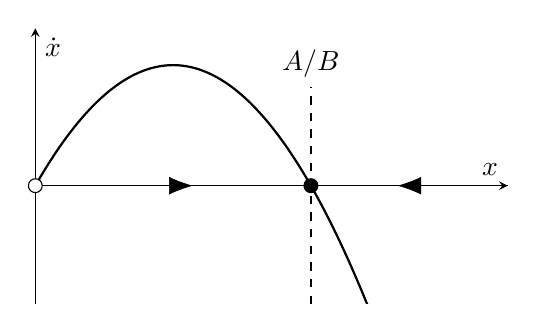
\begin{tikzpicture}
            \pgfplotsset{ticks=none},
            \begin{axis} [
                    ymax=4,
                    ymin=-3,
                    xmax=6,
                    xmin=-0.09,
                    x=1cm,
                    y=0.5cm,
                    axis lines=center,
                    trig format plots=rad,
                    ylabel={$\dot{\fcn}$},
                    xlabel={$\fcn$}
                ]
                \addplot [domain=0:6, samples=100, smooth, thick] { 3.5*x - x^2 };

                \draw[-{Latex[length=3mm]}, very thin] (axis cs:6,0) -- (axis cs:4.6,0);
                \draw[-{Latex[length=3mm]}, very thin] (axis cs:0,0) -- (axis cs:2,0);

                \node[circle, draw=black, fill=white, inner sep=0pt, minimum size=5pt] at (axis cs:0,0) {};
                \node[circle, draw=black, fill=black, inner sep=0pt, minimum size=5pt] at (axis cs:3.5,0) {};

                \draw[thick, dashed]
                (axis cs: 3.5, -3) to (axis cs: 3.5, 2.5) coordinate[label = {above:$A/B$}];
            \end{axis}
        \end{tikzpicture}
    \end{center}
    Når høyresiden i ligning \eqref{eq:populasjonsmodell} er positiv, altså for
    \begin{equation*}
        0 < \fcn(t) < \frac{A}{B},
    \end{equation*}
    er den deriverte også positiv, og populasjonen øker. Dersom populasjonen $\fcn(t)$ overstiger $A/B$ antall individer ser vi fra diagrammet at populasjonen begynner å minke, siden den deriverte nå er negativ (dette er tegnet inn som piler langs den horisontale aksen i diagrammet). Ut fra dette kan vi forvente oss at en hvilken som helst populasjon som følger loven \eqref{eq:populasjonsmodell} vil bevege seg mot likevektspunktet $\fcn(t) = A/B$. Dette likevektspunktet er stabilt, siden pilene fra begge sider peker inn mot dette punktet. I $\fcn = 0$ har vi et ustabilt likevektspunkt, ettersom et hvert avvik fra null medlemmer vil gjøre at populasjonen øker, helt til den når likevektspunktet i $A/B$.
\end{ex}

Diagrammet som ble brukt i Eksempel \ref{eks:populasjon_2} er et enkelt eksempel på et fasediagram. I stedet for å plotte løsningen $\fcn(t)$ mot variabelen $t$ plotter vi i fasediagrammet den deriverte $\dot{\fcn}$ mot $\fcn$ selv. Variabelen $t$ er dermed bare implisitt tilstede i fasediagrammet. Analysen består i å identifisere likevektspunktene til systemet, altså verdier for $\fcn$ slik at $\dot{\fcn} = 0$, for så å resonnere seg frem til for hvordan $\fcn(t)$ beveger seg mellom disse.


\section*{Eksistens og entydighet}

Vi skal nå se på hva som kan sies om eksistens og entydighet av løsninger for det generelle initialverdiproblemet
\begin{equation} \label{eq:ivp_2}
    \left\{
    \begin{aligned}
         & \dot{\fcn} = f(t, \fcn), \\
         & \fcn(t_0) = \fcn_0.
    \end{aligned}
    \right.
\end{equation}
Dette kan virke litt umotivert for øyeblikket, fordi vi til nå bare har sett et lite utvalg av veldig snille ligninger. I det generelle tilfellet er det ofte svært vanskelig, og noen ganger umulig, å finne entydige løsninger til problemet \eqref{eq:ivp_2}. Derfor inkluderer vi følgende resultat, som gir betingelser for eksistens og entydighet av løsninger.

\begin{thm} \label{thm:eksistens_unikhet}
    La $f(t, x)$ være en kontinuerlig funksjon på en åpen mengde $U \subset \mathbb{R}^2$ slik at $(t_0, x_0) \in U$, og anta at $f$ er kontinuerlig deriverbar i variabelen $x$ på området $U$. Da eksisterer det et tall $\delta > 0$ og en entydig løsning $x(t)$ til initialverdiproblemet \eqref{eq:ivp_2} på intervallet ${I = [t_0 - \delta, t_0 + \delta]}$.
\end{thm}

Tidligere har vi brukt fikspunktiterasjon til å løse skalare ligninger numerisk. Nå skal vi ta dette et steg videre, ved å løse initialverdiproblemet \eqref{eq:ivp_2} med fikspunktiterasjon. Beviset her er kun en skisse av de viktigste ideene, mens detaljene er utelatt. Vi må likevel introdusere følgende fakta som argumentasjonen er avhengig av. Dersom $g(x)$ er en kontinuerlig funksjon på et lukket intervall $I$ finnes det en konstant $L < \infty$ slik at
\begin{equation*}
    \max_{x \in I} \abs{f(x)} \leq L.
\end{equation*}
Videre, dersom $g$ er kontinuerlig deriverbar på et lukket intervall $I$ gjelder midellverditeoremet for funksjonen $g$, og vi har
\begin{equation} \label{eq:lip}
        \abs{g(x) - g(y)} \leq \max_{x \in I} \bigabs{f'(x)} \abs{x-y} \leq L \abs{x-y},
\end{equation}
for alle $x, y \in I$, siden den deriverte av $f$ er kontinuerlig.

\begin{proof}[Skisse av bevis for Teorem \ref{thm:eksistens_unikhet}]
    Som vist ovenfor kan initialverdiproblemet \eqref{eq:ivp_2} skrives på integralform
    \begin{equation*}
        x(t) = x(t_0) + \int_{t_0}^t f(s, x(s)) \diff{s}.
    \end{equation*}
    Med dette som utgangspunkt kan vi definere fikspunktiterasjonen
    \begin{equation}
        g_{n+1}(t) = \fcn_0 + \int_{t_0}^{t} f(s, g_n(s)) \diff{s},
    \end{equation}
    som gir opphav til en følge funksjoner $\{g_n(t)\}_{n \in \mathbb{N}}$. Merk at dette er en utvidelse av fikspunktalgoritmene vi har sett tidligere: dette er en rekursiv formel for funksjoner, og ikke tall. La oss nå anta at vi begynner med konstanten $x_0$ som $g_0(t)$, altså vår første gjetning på hva løsningen er. Da blir
    \begin{equation*}
        g_1(t) = \fcn_0 + \int_{t_0}^{t} f(s, x_0) \diff{s}.
    \end{equation*}
    Hvor stor er forskjellen mellom $g_0(t)$ og $g_1(t)$? Differansen i den første rekursjonen på et intervall $I$ rundt $t_0$ blir
    \begin{equation*}
        \begin{aligned}
            \abs{g_1(t) - g_0(t)} = & \biggabs{x_0 + \int_{t_0}^{t} f(s, x_0) \diff{s} - x_0} \\
            & = \biggabs{ \int_{t_0}^{t} f(s, x_0) \diff{s} } \\
            & \leq \int_{t_0}^{t} \abs{f(s, x_0)} \diff{s} \\
            & \leq \abs{t - t_0} \max_{t \in I} \bigabs{f(t, x_0)}.
        \end{aligned}
    \end{equation*}
    Siden $f$ er kontinuerlig på en mengde $U$ som inneholder $(t_0, x_0)$ kan vi anta at $f$ er kontinuerlig på intervallet $I = [t_0 - \delta, t_0 + \delta]$ (ved å velge $\delta$ liten), slik at
    \begin{equation*}
        \max_{t \in I} \bigabs{f(t, x_0)} \leq L < \infty.
    \end{equation*}
    Vi har også at $\abs{t - t_0} \leq \delta$ for $t \in I$. Dermed har vi
    \begin{equation} \label{eq:første_diff}
        \abs{g_1(t) - g_0(t)} \leq \abs{t - t_0} \max_{t \in I} \bigabs{f(t, x_0)} \leq \delta L.
    \end{equation}
    Den neste differansen i rekursjonen blir da
    \begin{equation*}
        \begin{aligned}
            \abs{g_{2}(t) - g_1(t)} & = \biggabs{\int_{t_0}^{t} f(s, g_1(s)) \diff{s} - \int_{t_0}^{t} f(s, g_{0}(s)) \diff{s}} \\
            & \leq \int_{t_0}^{t} \bigabs{f(s, g_1(s)) - f(s, g_{0}(s))} \diff{s} \\
            & \leq \int_{t_0}^{t} L \abs{g_1(s) - g_{0}(s)} \diff{s} \\
            & \leq \delta L^2 \int_{t_0}^{t} \diff{s} \\
            & \leq (\delta L)^2,
        \end{aligned}
    \end{equation*}
    der vi har brukt at ulikheten \eqref{eq:lip} siden $f$ er kontinuerlig deriverbar i $x$, og estimatet \eqref{eq:første_diff} for differansen $\abs{g_1 - g_0}$. Dette argumentet kan vi nå iterere i det uendelige, og neste differanse blir
    \begin{equation*}
        \begin{aligned}
            \abs{g_{3}(t) - g_2(t)} & = \biggabs{\int_{t_0}^{t} f(s, g_2(s)) \diff{s} - \int_{t_0}^{t} f(s, g_{1}(s)) \diff{s}} \\
            & \leq \int_{t_0}^{t} \abs{f(s, g_2(s)) - f(s, g_{1}(s))} \diff{s} \\
            & \leq \int_{t_0}^{t} L \abs{g_2(s) - g_{1}(s)} \diff{s} \\
            & \leq (\delta L)^3.
        \end{aligned}
    \end{equation*}
    Vi kan gjette på at den generelle sammenhengen blir
    \begin{equation*}
        \abs{g_{n+1}(t) - g_n(t)} \leq (\delta L)^n,     
    \end{equation*}
    noe fører oss til kjernen av argumentet: Dersom vi velger $\delta$ liten, slik at $\delta L < 1$, kommer differansen $\abs{g_{n+1}(t) - g_n(t)}$ til å bli mindre og mindre for større $n$. Vi har faktisk at ${(\delta L)^n \rightarrow 0}$ for ${n \rightarrow \infty}$ når $\delta L < 1$. Dette betyr at forskjellen blir mindre og mindre: det kan se ut som om følgen vår kommer til å konvergere! 
    
    Matematikere bruker også dette til å vise at følgen $\{g_n(t)\}_{n \in \mathbb{N}}$ konvergerer til en funksjon $g$, og at denne nødvendigvis løser initialverdiproblemet \eqref{eq:ivp} på intervallet $I$. Vi skal ikke gjøre dette grundig her, men med litt trening og litt mer kunnskap om konvergens i funksjonsrom kan du kanskje finne ut av detaljene selv.
\end{proof}

Teorem \ref{thm:eksistens_unikhet} er ofte greit å kjenne til, men kan ha begrenset praktisk betydning for en ingeniør. Som regel bruker vi numeriske metoder for å utforske differensialligninger.


\section*{Numeriske metoder}

Problemet vi står overfor er å finne en tilnærming til løsningen $\fcn(t)$ av initialverdiproblemet
\begin{equation} \label{eq:ivp_3}
    \left\{
    \begin{aligned}
         & \dot{\fcn} = f(t, \fcn(t)), \\
         & \fcn(t_0) = \fcn_0,
    \end{aligned}
    \right.
\end{equation}
på intervallet $[t_0, T]$, for $T > t_0$. La $\{t_i\}_{i = 0, ..., N}$ være en jevn partisjon
\begin{equation*}
    t_i = t_0 + h i, \qquad i = 0, 1, 2, ..., N
\end{equation*}
av intervallet $[t_0, T]$ i $N$ like lange delintervaller $[t_i, t_{i+1})$ av lengde
\begin{equation*}
    h = \frac{T - t_0}{N}.
\end{equation*}
Vi ønsker å approksimere funksjonen $\fcn(t)$ i punktene $t_i$, og innfører notasjonen $\fcn_i \approx \fcn(t_i)$ for tilnærmingen. Dette kan illustreres som vist under.
\begin{center}
    \begin{tikzpicture}
        \draw[thick, ->]
        (0, -0.1) to (0, 4) coordinate[label = {left:$\fcn(t)$}];
        \draw[thick, ->]
        (-0.1, 0) to (8, 0) coordinate[label = {below:$t$}];
        \draw[thick]
        (1, 0.3) to (1, -0.3) coordinate[label = {below:$t_0$}];
        \draw[thick]
        (2, 0.3) to (2, -0.3) coordinate[label = {below:$t_1$}];
        \draw[thick]
        (3, 0.3) to (3, -0.3) coordinate[label = {below:$t_2$}];
        \draw[thick]
        (5, 0.3) to (5, -0.3) coordinate[label = {below:$t_i$}];
        \draw[thick]
        (7, 0.3) to (7, -0.3) coordinate[label = {below:$T$}];

        \draw (4, -0.2) coordinate[label = {below:$\cdots$}];
        \draw (5.2, 1.1) coordinate[label = {above:$\fcn_i \approx \fcn(t_i)$}];

        \filldraw[black] (1, 3) circle (1pt) coordinate[label = {above:$\fcn_0$}];
        \filldraw[black] (2, 2) circle (1pt) coordinate[label = {above:$\fcn_1$}];
        \filldraw[black] (3, 1.5) circle (1pt) coordinate[label = {above:$\fcn_2$}];
        \filldraw[black] (5, 1) circle (1pt);
        \filldraw[black] (7, 0.8) circle (1pt) coordinate[label = {above:$\fcn_N$}];
        
        \draw[decoration={brace},decorate]
        (1,0.4) -- node[above=5pt] {$h$} (2, 0.4);
    
    \end{tikzpicture}
\end{center}

For å utlede formler for tilnærmingen $\{\fcn_i\}_{i = 0, ..., N}$ for $\fcn(t)$ kan vi integrere initialverdiproblemet \eqref{eq:ivp_3} over et delintervall $[t_i, t_{i+1})$, noe som gir
\begin{equation*}
    \fcn(t_{i+1}) - \fcn(t_i) = \int_{t_i}^{t_{i+1}} f(s, \fcn(s)) \diff{s}.
\end{equation*}
Dette gir formelen
\begin{equation*}
    \fcn_{i+1} \approx \fcn_i + \int_{t_i}^{t_{i+1}} f(s, \fcn(s)) \diff{s},
\end{equation*}
som kan regnes ut ved numerisk approksimasjon av integralet på høyre side. Vi lister opp noen ulike måter å gjøre dette på.

Den enkleste tilnærmingen er å anta at $f(t, \fcn(t)) \approx f(t_i, \fcn_i)$ på $[t_i, t_{i+1})$. Det gir
\begin{equation*}
    \int_{t_i}^{t_{i+1}} f(s, \fcn(s)) \diff{s} \approx \int_{t_i}^{t_{i+1}} f(t_i, \fcn_i) \diff{s} = h f(t_i, \fcn_i),
\end{equation*}
som gir opphav til Eulers eksplisitte metode
\begin{equation*}
    \fcn_{i + 1} = \fcn_i + h f(t_i, \fcn_i), \qquad i = 0, \cdots, N - 1.
\end{equation*}
Med tilnærmingen
\begin{equation*}
    \int_{t_i}^{t_{i+1}} f(\fcn(s), s) \diff{s} \approx h f(t_{i+1}, \fcn_{i+1})
\end{equation*}
får vi Eulers implisitte metode, mens trapesregelen for integraler
\begin{equation*}
    \int_{t_i}^{t_{i+1}} f(\fcn(s), s) \diff{s} \approx \frac{h}{2} (f(t_{i}, \fcn_{i}) + f(t_{i+1}, \fcn_{i+1}))
\end{equation*}
gir trapesmetoden. Dersom vi i trapesmetoden tilnærmer $\fcn_{i+1}$ med Eulers eksplisitte metode får vi Heuns metode. Til sist, ved approksimasjonen
\begin{equation*}
    \int_{t_i}^{t_{i+1}} f(\fcn(s), s) \diff{s} \approx h f\bigparanth{\frac{t_{i+1} + t_i}{2}, \frac{\fcn_{i+1} + \fcn_i}{2}}
\end{equation*}
får man midtpunktmetoden.


\begin{defn}
    Vi har nå definert følgende numeriske metoder for initialverdiproblemet \eqref{eq:ivp_3} over partisjonen $\{t_i\}_{i = 0, ..., N}$ av $[t_0, T]$.
    \begin{align}
        \fcn_{i + 1} & = \fcn_i + h f(t_i, \fcn_i), \tag{Euler eksplisitt} \\
        \fcn_{i + 1} & = \fcn_i + h f(t_{i+1}, \fcn_{i+1}), \tag{Euler implisitt} \\
        \fcn_{i + 1} & = \fcn_i + \frac{h}{2} (f(t_{i}, \fcn_{i}) + f(t_{i+1}, \fcn_{i+1})), \tag{trapesmetoden} \\
        \fcn_{i + 1} & = \fcn_i + h f\biggparanth{\frac{t_{i+1} + t_i}{2}, \frac{\fcn_{i+1} + \fcn_i}{2}}, \tag{midtpunktmetoden}
    \end{align}
    og
    \begin{equation} \tag{Hens metode}
        \left\{
            \begin{aligned}
                \fcn^* & = \fcn_i + h f(t_i, \fcn_i), \\
                \fcn_{i + 1} & = \fcn_i + \frac{h}{2} (f(t_{i}, \fcn_{i}) + f(t_{i+1}, \fcn^*)).
            \end{aligned}
            \right.
        \end{equation}
\end{defn}
        
Har det noe å si hvilken metode vi bruker? La oss sammenligne metodene på et testproblem.

\begin{ex} \label{eks:testproblem_numerikk}
    Vi anvender metodene over til å løse initialverdiproblemet
    \begin{equation*}
        \left\{ 
            \begin{aligned}
                & \dot{\fcn} = - \fcn, \\
                & \fcn(0) = 1,
            \end{aligned}
        \right.
    \end{equation*}
    på intervallet $[0, 1]$, med steglengde $h = 0.25$. Resultatet vises i figuren under.
    \begin{center}
        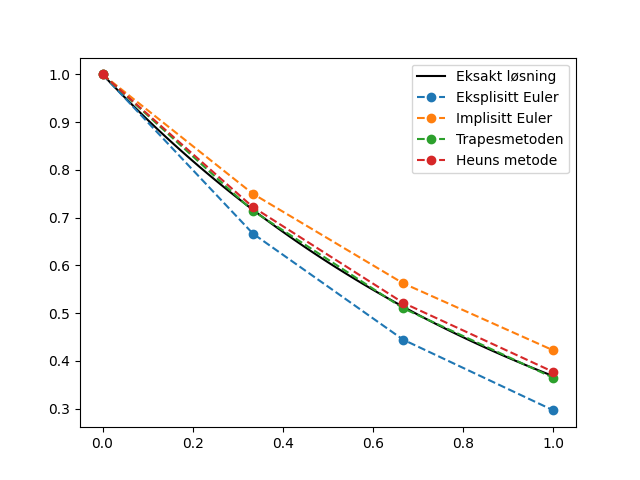
\includegraphics[scale=0.6]{methods_test.png}
    \end{center}
    Nå endrer vi på steglengden $h$, og ser hvordan feilen i forhold til den eksakte løsningen endrer seg. Den lokale feilen, altså differansen $\abs{\fcn(t_1) - \fcn_1}$ for første steg, er vist for de ulike metodene i følgende tabell.
    \begin{center}
        \begin{tabular}{c | c | c | c | c}
            $h$ & Euler eksplisitt & Euler implisitt & Trapesmetoden & Heuns metode \\
            \hline
            $10^{-1}$ & $5.950e-03$ & $5.161e-03$ & $1.025e-04$ & $2.224e-04$ \\
            $10^{-2}$ & $5.084e-05$ & $5.017e-05$ & $8.502e-08$ & $1.713e-07$ \\
            $10^{-3}$ & $5.008e-07$ & $5.002e-07$ & $8.350e-11$ & $1.671e-10$ \\
            $10^{-4}$ & $5.001e-09$ & $5.000e-09$ & $8.338e-14$ & $1.668e-13$
        \end{tabular}
    \end{center}
    Her observerer vi at for Eulers eksplisitte og implisitte metode blir feilen omtrent hundre ganger mindre dersom vi gjør steglengden ti ganger mindre, mens for trapesmetoden og Heuns metode kan det se ut som om feilen blir tusen ganger mindre hver gang vi gjør steglengden ti ganger mindre.

    Den globale feilen, altså feilen $\abs{\fcn(t_N) - \fcn_N}$ i siste steget, finner vi som gitt i tabellen under.
    \begin{center}
        \begin{tabular}{c | c | c | c | c}
            $h$ & Euler eksplisitt & Euler implisitt & Trapesmetoden & Heuns metode \\
            \hline
            $10^{-1}$ & $2.144e-02$ & $1.954e-02$ & $3.790e-04$ & $8.237e-04$ \\
            $10^{-2}$ & $1.866e-03$ & $1.850e-03$ & $3.128e-06$ & $6.303e-06$ \\
            $10^{-3}$ & $1.842e-04$ & $1.840e-04$ & $3.072e-08$ & $6.148e-08$ \\
            $10^{-4}$ & $1.840e-05$ & $1.840e-05$ & $3.069e-10$ & $6.133e-10$
        \end{tabular}
    \end{center}
    Her ser vi at feiler minsker proporsjonalt med steglengden for eksplisitt og implisitt Euler, mens den minsker kvadratisk med steglengden for trapesmetoden og Heuns metode.
\end{ex}


\section*{Analyse av numeriske metoder}

Målet er nå å forklare mønsteret vi observerte i tabellene fra Eksempel \ref{eks:testproblem_numerikk}. Til dette formål er hovedverktøyet vårt Taylorutviklingen
\begin{equation} \label{eq:taylor}
    \fcn(t + h) = \sum_{i=0}^n \frac{h^n}{n!}\fcn^{(n)}(t) = \fcn(t) + h \dot{\fcn}(t) + \frac{h^2}{2} \ddot{\fcn}(t) + \cdots
\end{equation}
av løsingen $\fcn(t)$. Merk at denne formelen er en antagelse vi må gjøre, siden vi ikke på forhånd vet at $\fcn(t)$ er en glatt funksjon og derfor kan utvlikles som en rekke i henhold til Taylors teorem. I praksis fungerer likevel dette bra.

Vi utleder den lokale feilen i Eulers eksplisitte metode. Først antar vi at $\fcn_i = \fcn(t_i)$, altså at approksimasjonen er lik den eksakte løsningen i punktet $t_i$. Så ønsker vi å se på differansen mellom den eksakte løsningen og approksimasjonen i neste steg, altså
\begin{equation*}
    \varepsilon_i := \fcn(t_i + h) - \fcn_{t_{i+1}}.
\end{equation*}
Ved hjelp av rekkeutviklingen \eqref{eq:taylor} finner vi
\begin{equation*}
    \begin{aligned}
        \varepsilon_i & = \fcn(t_i + h) - \fcn_{t_{i+1}} \\
        & = \fcn(t_i) + h \dot{\fcn}(t_i) + \frac{h^2}{2} \ddot{\fcn}(t_i) + \bigo{h^3} - \fcn_i - h f(t_i, \fcn_i) \\
        & = \fcn(t_i) - \fcn_i + h f(t_i, \fcn_i) - h f(\fcn_i, t_i) + \frac{h^2}{2} \ddot{\fcn}(t_i) + \bigo{h^3} \\
        & = \frac{h^2}{2} \ddot{\fcn}(t_i) + \bigo{h^3}
    \end{aligned}
\end{equation*}
der vi har brukt at $\fcn(t_i) = \fcn_i$ og at $\dot{\fcn}(t_i) = f(t_i, \fcn_i)$. For liten steglengde $h$ øker derfor feilen maksimalt som $h^2$ på dette ene steget, akkurat som observert i Eksempel \ref{eks:testproblem_numerikk}.

Vi kan forvente å få et estimat på den globale feilen dersom vi ser på summen av de lokale feilene. Det gir
\begin{equation*}
    \mathcal{E} := \sum_{i = 0}^N \varepsilon_i \leq \sum_{i = 1}^N \bigabs{\frac{h^2}{2}\ddot{\fcn}(t_i)} \leq \frac{M h^2}{2} N = \bigo{h},
\end{equation*}
der vi har antatt at $\ddot{\fcn} \leq M$ på $[t_0, T]$ (to ganger kontinuerlig deriverbar). Dette er også i overensstemmelse med Eksempel \ref{eks:testproblem_numerikk}.

Til slutt skal vi se på én fordel og én ulempe med implisitte metoder som kan være greit å vite om.

\begin{ex}
    Igjen ser vi på problemet
    \begin{equation*}
        \left\{ 
            \begin{aligned}
                & \dot{\fcn} = - \fcn, \\
                & \fcn(0) = 1,
            \end{aligned}
        \right.
    \end{equation*}
    men denne gangen på intervallet $[0, 15]$. Euler eksplisitt og Euler implisitt på problemet, med steglengde $h = 3$, produserer følgende approksimasjoner til løsningen.
    \begin{center}
        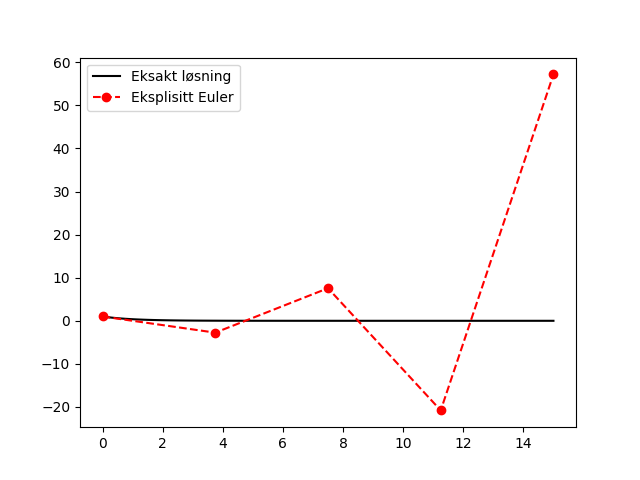
\includegraphics[width=0.48\textwidth]{stability_test_explicit.png}
        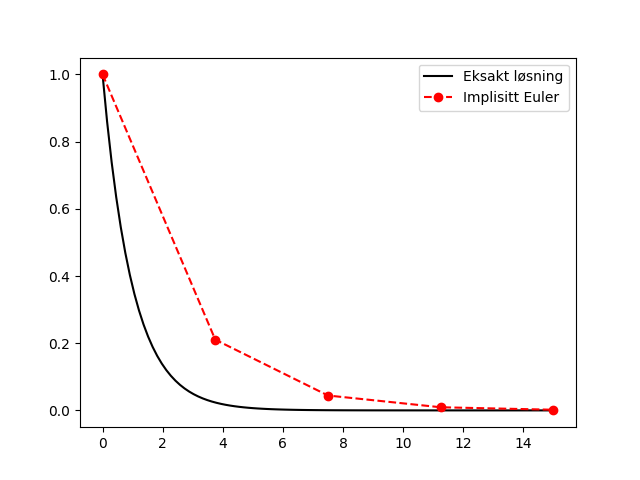
\includegraphics[width=0.48\textwidth]{stability_test_implicit.png}
    \end{center}
    Her kan man tydelig se at den implisitte metoden fungerer mye bedre enn den eksplisitte: den implisitte metoden virker å være mer stabil. Erfaring tilsier at implisitte metoder som regel er mye mer robuste når det kommer til stabilitet.
\end{ex}

\begin{ex}
    Vi prøver oss på problemet
    \begin{equation*}
        \left\{
        \begin{aligned}
            & \dot{\fcn} = \sin(\fcn), \\
            & \fcn(0) = \frac{\pi}{4}.
        \end{aligned}
        \right.
    \end{equation*}
    Eulers implisitte metode med steglengde $h$ blir
    \begin{equation*}
        \fcn_{i + 1} = \fcn_i + h \sin(\fcn_{i+1}).
    \end{equation*}
    Men denne ligningen kan ikke løses eksplisitt for $\fcn_{i+1}$! Det betyr at for hvert steg må vi beregne $\fcn_{i+1}$ med en numerisk ligningsløser, som f.eks fikspunktiterasjon eller Newtons metode. Dette kan gjøre implisitte metoder mer tidkrevende enn eksplisitte metoder.
\end{ex}


\end{document}
